
\chapter{Design}

%\subsubsection{Recording user interactions}


\begin{itemize}
    \item In this chapter, we design our history system.
    \item The resulting design we present in this chapter is a result of iterative process based on experiments and feedback from users. Designing user interfaces without iterative design often leads to usability issues.\cite{nielsen1993iterative}
    \item (When designing new features to be integrated into shell ...) People are used to standard history features. We need to respect the habits that people built while using them. This is true for any design but it is especially important for features integrated into shell. Discoverability is very bad in shell because available features are invisible.\footnote{For example, if we design a new history tool and bind it to an unused key, there is not really a way for our users to discover it. Compare this with GUI applications where available features can be displayed on the screen.}
    \item We also want to keep the design simple so that the user is not overwhelmed with available features. According to \cite{greenberg1993computer}, overloading history mechanisms with complex functionality would not make them better.
    \item the structure
    \subitem We introduce requirements that are based on previous analysis
    \subitem We describe the features we want in the design
    \subitem We explain the architecture of the history system, describe the parts and their responsibilities
    \subitem We design the interactive parts of the system - the behavior we want the user to experience
    \subitem We describe the backend parts of the system - the necessary processes
    \subitem We show and explain the communication that needs to happen between parts of the system
    \subitem Finally, we come back to the requirements and we explain how each of them is fulfilled
\end{itemize}





\newpage
\section{Requirements and features}


The requirements we selected based on the previous analysis are following:

\begin{itemize}
\item Record shell history with context and usage
% \item Allow unlimited history
\item Allow history sharing between open sessions
\item Provide good out-of-the-box experience
\subitem Allow people to use the history system without configuring it first
\subitem Allow use of the system without reading manuals or help pages
\item Respect existing history features and existing habits of people
\subitem Do not change keybindings used to complete existing workflows
\subitem Support original workflows when replacing history mechanisms
\item Provide a replacement for reverse search
\subitem Solve the issues with standard reverse search
\subitem Match the few main improvements offered by Hstr and Fzf
\subitem Use recorded context to enhance history searching capabilities
\item Provide support for sequence repeating (forward in history)
\item Provide support for synchronization of shell history between devices
\item Provide support for contextual autosuggestions
\end{itemize}



\subsection{Basic features}

Now, we describe the basic features of the design. These features might seem obvious, but we point them out because they do contribute to the resulting usefulness of the history system.

History should be collected and recorded in a robust way; History should be unlimited, and using multiple simultaneous sessions must not result in missing history entries. 
Simultaneous sessions should be handled is a way that allows accessing history from other sessions.
All this has to work by default; No configuration should be necessary to achieve the basic functionality. 

The default configuration should provide good out-of-the-box experience for the average target user. It should not be necessary to read help pages or manuals to make use of the history system's main features. 
All new features should take the original habits of people into account. 
Introducing new or changing meaning of existing key bindings should be done with care. It is not easy for people to discover new key bindings in the shell.


\subsection{Core features}

The core focus of this design is providing a replacement for the standard reverse search. In this section, we explain why we chose this as the main focus of the design. We discuss how it relates to standard shell history features, existing state-of-the-art history tools, and possibilities of enhancing history searching with context.

%\paragraph{Standard history features}

Standard history features form the base that people are used to. We should not redesign and replace them unless we have a good reason to.
As we saw in the analysis, the standard reverse search does not provide a good feature set to complete many workflows. Furthermore, there are other tools available that provide features that solve the issues of reverse search. Because of this, we design a searching application that replaces and improves the reverse search.

%For example, we have no reason to change history expansion. Accessing recent history entries using \verb|ARROW_UP| works reasonably well in many situations. Furthermore, people expect \verb|ARROW_UP| to give them immediately previous history entries. Because of these reasons, we do not redesign \verb|ARROW_UP|.

% In contrast

%\paragraph{Matching the state-of-the-art}

Hstr\cite{toolshstr} and Fzf\cite{tools-fzf} are existing projects that replace reverse search and provide improved searching capabilities. 
Standard reverse search only uses a single query for searching and displays a single result at a time. In contrast, both of the tools mentioned above allow using more than a single query for searching and show a full screen of history results. We use these tools as an inspiration. Our searching application should match the key improvements provided by Hstr and Fzf. 

%\paragraph{Enhancing history searching with context}

%In analysis, we have identified workflows that are directly related to context. 
%Additionally, we described different ways how context relates to shell usage. 

In addition to matching the state-of-the-art features, we want to use context to enhance the searching capabilities of our history system. Our searching application should make it easier to retrieve history that matches the current context. 
% todo: do not be as specific CUT here


%This means that history entries from current directory, git repository, and host should be prioritized.
%In contrast, history entries with errors should be penalized.
%The relevant context should be visible when it affects the order of results.
%However, the user interface should not be cluttered with irrelevant context. 



\subsection{Additional features}

In this section, we cover features that are not the main focus of our design. These features are not as important as providing a replacement for the reverse search. However, they are still valuable, and we want to make sure they fit with the rest of the design. 
The chosen additional features are Forward in history, synchronizing history between devices, and Fish-like Autosuggestions.



%\paragraph{Forward in history}

Forward in history is a feature we can find in Python console in Blender. We adopt this feature into our design because it allows the user to easily repeat sequences of history entries. Support for repeating sequences from history is poor in standard shell history.

%\paragraph{Synchronizing history}

Synchronizing history between multiple devices is an appealing feature. It enables history reuse between devices. The potential for reuse is further enhanced by using context to prioritize the search results.
Synchronized history is also harder to lose because it is replicated across multiple devices. 

%\paragraph{Autosuggestions}

Autosuggestions are a very convenient and very fast history mechanism. Original Fish autosuggestions use context to determine what history entry should be displayed.
We want to include a similar feature in our design.

\newpage
\section{Architecture}

In the previous sections, we listed all the features that we chose to include in the design. We chose a set of features that fits well together and should significantly improve the usefulness of shell history.

Now, we design the architecture of our history system so that it can accommodate all the features. 
Our history system consists of a daemon and multiple components. The daemon is always running in the background. Components are integrated into the shell and activated at appropriate times. 

%\paragraph{Daemon}

Daemon allows us to asynchronously preprocess the history data and serve it to the components when it is needed. It is responsible for loading and saving history to the storage. Daemon gives us the option to easily share history between sessions. History synchronizations is initiated and controlled by the daemon.

%\paragraph{Components}

Multiple different components are activated at various times based on their purpose. The history collector records the shell history with context and sends it to the daemon. Autosuggestion and arrow keys handlers respond to the interactions with the user. Finally, the search application interacts with the user, communicates with the daemon, and does its own share of data processing.


For the purpose of this design, we divide the system into two logical sections: frontend and backend. As you can see in figure \ref{design-architecture-layers}, the frontend is responsible for the interactions with the shell, terminal, and by extension, the user. Backend is mostly about handling data. 

\begin{figure}[h!]
\centering
\tmpframe{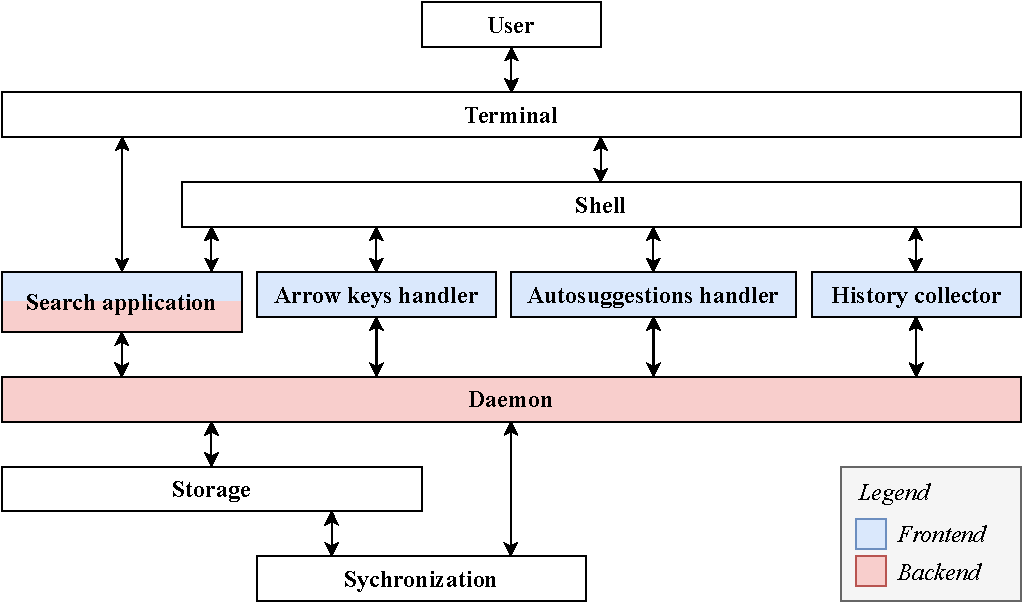
\includegraphics[width=\linewidth]{figures/design/thesis-design-architecture-layers-v2.pdf}}
\caption{Schema of architecture and communication}
\label{design-architecture-layers}
\end{figure}

\newpage
\section{Frontend}\label{design-frontend}

In this section, we focus on and design the parts of the system that the user interacts with. 
To relate this to our previous analysis, these are the specific workflows we are addressing in this section:

\begin{itemize}
\item Searching with limited knowledge (section \ref{workflow-search-w-limited-knowledge})
\item Searching with implicit context (section \ref{workflow-search-w-implicit-context})
\item Repeating a sequence of history entries (section \ref{workflow-repeating-a-sequence})
\end{itemize}

\subsection{Search application}

The most important part of our design is the replacement for standard reverse search -- a full-screen terminal history searching application. The application is inspired by Hstr and Fzf. 

We start by designing the visual layout of the application.
The wireframe in figure \ref{wireframe-normal} shows the layout of the default view of the application. There are three sections in the wireframe:

\begin{itemize}
\item Search input
\item Main section with search results
\item Status bar with details and help
\end{itemize}




The search results in the main section are interactively updated as the user types into the search input. Table \ref{tab:design-columns} shows which context is always visible and which is only displayed when relevant. Git repository and exit status both share the same column ("FLAGS"). 

\begin{table}[h]
\centering
\begin{tabular}{lllll}
\hline \hline
Context & Header & When visible \\\hline
Time/date & TIME & always \\ 
Host & HOST: & only for history from other hosts \\ 
Directory & DIRECTORY & always \\ 
Git repository & FLAGS & only for history from this git repo. \\ 
Exit status & FLAGS & only non-zero exit status \\ 
Command line & COMMAND-LINE & always \\\hline \hline
\end{tabular}
\caption{Context and columns in the default view}
\label{tab:design-columns}
\end{table}

Host and directory also share a single column, but they do have separate headers. Columns are being dynamically resized to fit the data and to not waste space. Command line entry, host, and directory are shortened to fit the screen if necessary. 

Near the bottom of the screen, there is a status bar with details about the currently selected command and help. These details are displayed without any shortening, and the status bar is expanded to accomodate them. Under the command details, there is help that shows key bindings and other information.


The wireframe in figure \ref{wireframe-detail} shows the detail view. In this view, the user can see the details and surrounding history entries for a single command line entry. Each command line entry can appear in history multiple times; The user can switch between these occurrences. The next occurrence is partially displayed to make it easier to compare the surrounding history entries.


% \subsubsection{Modes (Context/RAW)} - added after user feedback

\paragraph{Key bindings}
When designing key bindings, it is essential to respect existing key bindings and to leverage what are the users already used to.
We want to avoid collisions with flow control keybindings so we do not use \verb|CTRL-S| and \verb|CTRL-Q|. Additionally, we do not reuse standard job control key bindings \verb|CTRL-Z|. 
Since we are replacing the reverse search, we are following many of its key bindings. The list of keybindings for our history search application follows:

\begin{itemize}
\item \verb|CTRL-R| to launch the search application from the command line
\item Type to search
\item \verb|ARROW_UP|/\verb|ARROW_DOWN| to select 
\item \verb|ARROW_RIGHT| to paste the selected entry to the command line for editing
\item \verb|ENTER| to execute the selected entry
\item \verb|CTRL-X| to show detail view for the selected entry
\item \verb|CTRL-C|/\verb|CTRL-D| to quit
\item \verb|CTRL-G| to abort and paste the current search query onto the command line
\end{itemize}


\paragraph{Scaling in larger terminals}

Both wireframes above both use the standard 80x25 character terminal size. In larger terminals, there is more space that can be used. Columns with hosts, directories, and command line entries stretch to make use of the extra space. The main section with search results becomes longer, and consequently, more history entries fit in the terminal. 

\paragraph{Colors}

Our application has a lot of information to display. 
Colors are used to highlight the information that influences the order of displayed results. To make it easier to differentiate between different types of information, they are highlighted using different colors. 
The red color is reserved for highlighting remote hosts and non-zero error status; This communicates to the user that these history entries might not work well.
Currently selected history entry is highlighted by inverting the foreground and background colors.


\begin{figure}[h!]
\permanentframe{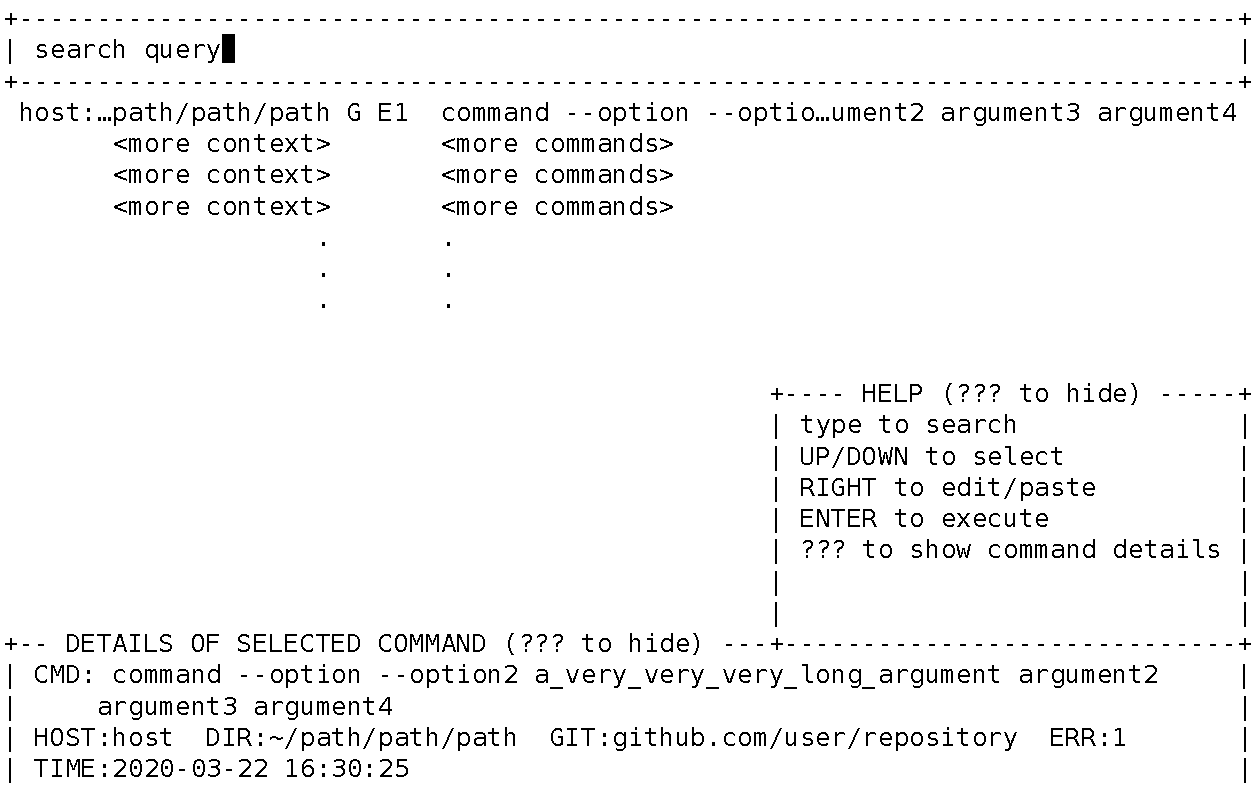
\includegraphics[width=0.995\linewidth]{figures/design/xterm-wireframe-bw-normal.pdf}}
\caption{Wireframe of default view}
\label{wireframe-normal}
\end{figure}

\begin{figure}[h!]
\permanentframe{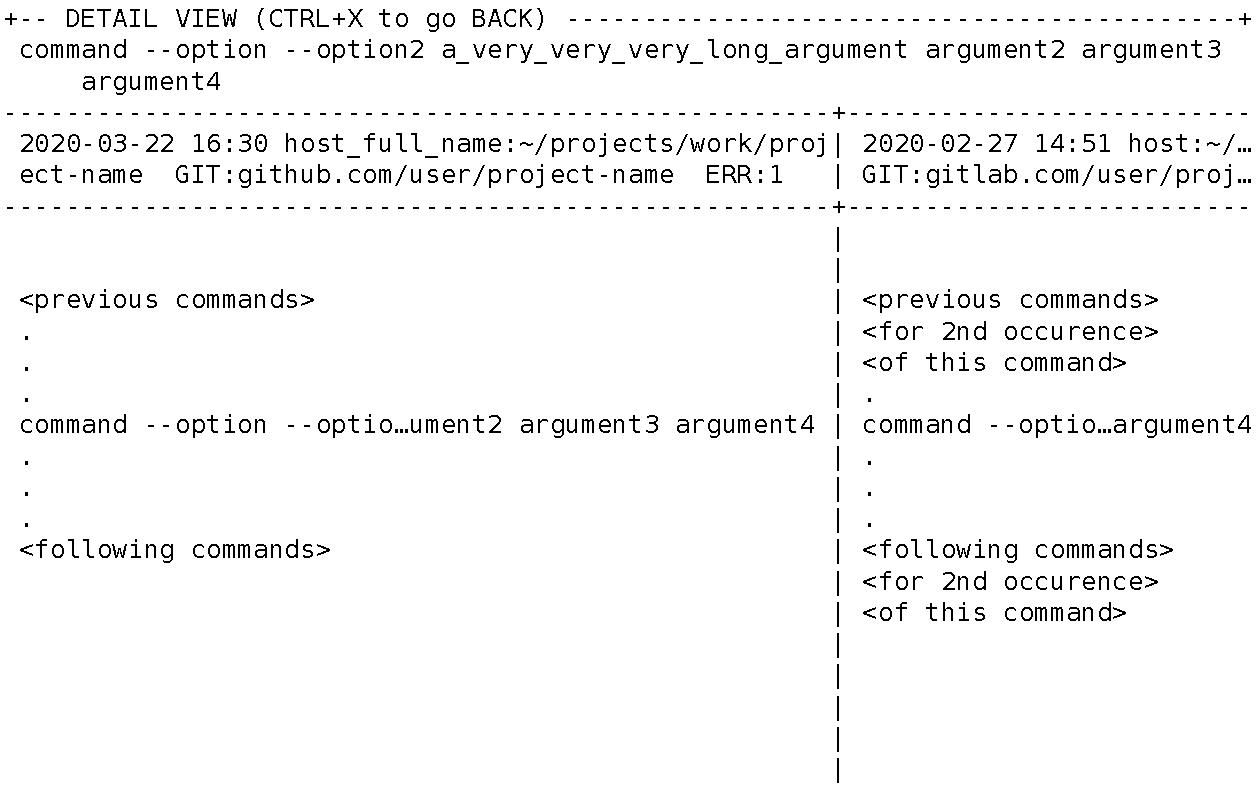
\includegraphics[width=0.995\linewidth]{figures/design/xterm-wireframe-bw-detail.pdf}}
\caption{Wireframe of detail view}
\label{wireframe-detail}
\end{figure}


\subsection{Arrow key handler}

Our previous analysis found out that standard history mechanisms available via arrow keys work reasonably well. Furthermore, people have a strong expectation of seeing recent history entries on \verb|ARROW_UP|. 
For these reasons, we only introduce minor changes into the standard behavior of arrow keys.


In our design, the prefix history search is enabled by default. It is a useful feature that does not interfere with the standard stepping through history. Additionally, the history available via \verb|ARROW_UP| is fully deduplicated.

\paragraph{Forward history}

In standard shell history, \verb|ARROW_DOWN| is without function unless we press \verb|ARROW_UP| first. It is only useful as a way to get back from recent history to the original command line.

We overload \verb|ARROW_DOWN| with an additional feature - Forward in history. When previously executed command line entry was retrieved from history, pressing \verb|ARROW_DOWN| gives the user access to the next history entry in the sequence. 
The user can easily repeat whole sequences because each history entry in the sequence can be retrieved by a single press of \verb|ARROW_DOWN| and then executed. 


To preserve the ability to hold \verb|ARROW_DOWN| to return from recent history to the original command line, we introduce a delay. A delay in activation of forward history feature that is triggered when the user holds down \verb|ARROW_DOWN| while in recent history.

\subsection{Autosuggestions handler}

Autosuggestions in our history system use the recorded context to recommend history entries to the user. The suggested history entry is determined based on the current context. History is searched for matching entries in this order:

\begin{itemize}
\item history from the current directory
\item history from the current git repository
\item history from the current host
\item history from anywhere
\end{itemize}

Additionally, we introduce an exception to enhance the Forward in history feature. 
When the user uses \verb|ARROW_DOWN| the next autosuggestion should try matching a few next history entries in the history sequence before any other history entries. 

\section{Backend}

In previous sections, we focused on the parts of the system user interacts with.
Now we design the inner workings of the system that make it possible to provide the desired behavior to the user.

\subsection{Search algorithm}

The terminal history searching application needs to serve relevant entries to the user based on the typed query and current context. When searching, each history record is assigned a score; This score is based on how well history record matches the query, how well it matches the current context, and also on its time of execution. 

After scoring all the history records, they are sorted. Finally, history entries with the highest scores are displayed to the user.

% It is essential to strike a good balance between effects of the query and the context. 
\paragraph{Scoring metric}

%Results that are displayed near the top ... is very important because it 
The score for a record \(r\) with query \(q\) and current context \(c\) is a sum of three parts: 

\[ Score_r(q,c) = w_1 \cdot QueryScore_r(q) + w_2 \cdot ContextScore_r(c) + w_3 \cdot TimeScore_r \]

The score weights \(w_1\), \(w_2\), and \(w_3\) determine how the parts of the score relate to each other. 

The first part, \(QueryScore\), represents how well the history record matches the query typed by the user. It is essential that \(QueryScore\) has the most influence over the total resulting score. Not giving enough weight to it could lead to situations where the user types in a query, but the displayed results match the context instead. 

The second most important part is \(ContextScore\); It represents the similarity between the context of the history record and the current context. Finally, \(TimeScore\) gives higher scores to more recent history entries. The influence of \(TimeScore\) on the total resulting score should be marginal.

Now that we covered how the partial scores relate to each other, we look at them individually.





\paragraph{Query score}

To calculate the \(QueryScore\), the query provided by the user is broken down into individual words. 
Each word is matched against the command line entries separately. Each query word also independently contributes to the score. This means that as the user adds more words to the query, the influence of the context becomes less and less significant.

We formalize this property as follows; Let queries \(q_1\) and \(q_2\) be represented as sets of individual words. For any queries \(q_1\), \(q_2\) and any history record \(r\): 

\[ q_1 \subset q_2 \Rightarrow QueryScore_r(q_1) \leq QueryScore_r(q_2)\]\

\paragraph{Context score}
The second part of the total score is \(ContextScore\); It takes the current context at the time of execution of the search application and compares it to the context of individual history records. 
The current context is compared with the context of the history records using four conditions displayed in the table \ref{tab:score-matching-context}. As shown in the table, each of these conditions either increases or decreases the score.

\begin{table}[h]
\centering
\begin{tabular}{lll}
\hline \hline
Context condition & Effect \\
\hline
Directory matches & significantly increase score \\ 
Git repository matches & increase score \\ 
Non-zero exit status & decrease score \\
Host does not match & slightly decrease score \\ 
\hline \hline
\end{tabular}
\caption{Influence of different parts of context on \(ContextScore\)}
\label{tab:score-matching-context}
\end{table}

To make it easy to skim over displayed results in the search application, we want the results to be grouped based on context when possible. 
We want to prevent history records with different contexts from being unnecessarily mixed together. 
To achieve that, \(ContextScore\) should be an injective function of the history record context.

In other words, any two history records \(r\) and \(s\) with different contexts never share the same \(ContextScore\) for a given current context \(c\):
\[ context_{r} \neq context_{s} \Rightarrow ContextScore_r(c) \neq ContextScore_s(c) \]\
Here, \(context\) of history record \(r\) is defined as its directory, git repository, exit status, and host:
\[ context_r = (directory_r, gitRepository_r, exitStatus_r, host_r) \]



\paragraph{Time score}

The last part of the score is \(TimeScore\). It is the least important of the partial scores. The most recent entries have the highest \(TimeScore\), and older entries have lower \(TimeScore\). 



\paragraph{Score weights}

We described the scoring function as a whole. We also introduced some important properties of the partial scoring functions. However, the resulting behavior of the whole scoring function depends on the concrete weights we use. 
Specific weights should be determined experimentally based on real-life shell history.



%\subsection{Open session tracking}

%Features like forward in history need to quickly serve specific history entries to the user. This requires the necessary history records to be processed and held in memory. 
%Data processing is the responsibility of the daemon. Daemon keeps track of open sessions and prepares the necessary history records for them.


\subsection{History synchronization between devices}

Instead of implementing our own dedicated synchronization server, we design our history system to rely on third-party services for synchronization. 

The process of synchronization works like this: First, we check if there are any new history entries. If so, we download them and merge them into local history. Finally, we check for new history again, and if there is none, we upload the newly merged history. 

The daemon controls this whole synchronization process; It initiates the individual steps and handles when they fail. It also takes care of the history merging. Download, upload, and checking for new history is not part of the daemon. These three steps are different for each synchronization service; They are extracted out of the daemon and combined into a "Synchronization connector". Each synchronization connector provides support for a single synchronization method. Synchronization connectors do not contain any complicated logic. 


\subsection{Data representation}

In this section, we discuss what data we need to handle and how it should be represented so that all the chosen requirements and features are possible.


Contextual shell history is inherently relational; Each history record was executed as part of a given session, on a host, in a specific directory. However, we do not need the relational properties of the history for most of the features. For example, when searching, we need to calculate scores for all history entries, not just the ones with matching context. 

We represent the data as a stream of history records; Each record can be uniquely identified by its ID. Separate entries are very easy to merge when we synchronize history from multiple devices.

Based on all requirements and features of our design, each record has to contain at least following data:
\begin{itemize}
\item machine ID
\item session ID
\item record ID
\item time of execution
\item host
\item directory
\item git repository
\item exit status
\item command line entry
\item usage data / user interactions
\end{itemize}



\begin{figure}
\centering
\tmpframe{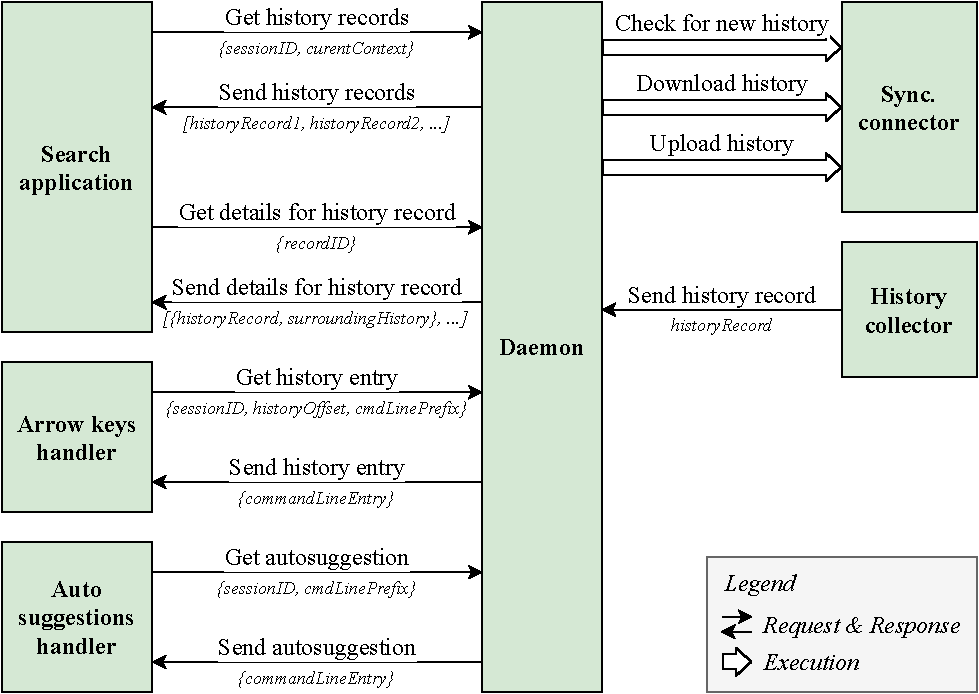
\includegraphics[width=\linewidth]{figures/design/thesis-design-api.pdf}}
\caption{Schema of communication and exchanged data}
\label{design-api}
\end{figure}


\subsection{Communication}

Here, we describe the communication between the components of our history system. Figure \ref{design-api} shows requests, responses, and execution that happen in the system. Data that is sent with each request is displayed under the arrow. 

The search application requests all history records when it is launched and then requests details for a specific history record when the user switches to the detail view. Response with the details for the history record contains a list of occurrences of the command line entry; Each occurrence consists of the history record and surrounding command line entries.

Arrow key handler is simpler; It requests a history entry based on the current session, the prefix that is already typed on the command line, and history offset that represents how many times did the user press the arrow key. The response is a single command line entry to display.

Autosuggestions handler requests a command line entry to show. The request contains a session ID and the prefix that the user already typed on the command line.

All of these components are integrated into the shell and activated when a specific key is pressed. Furthermore, they directly manipulate the contents of the command line when they return a command line entry to the user.

The history collector is also integrated into the shell so that it can collect the current context and send it to the daemon. Synchronization connector does not receive any data; instead, it is executed by the daemon to complete low-level synchronization tasks. 

\section{Design testing}

In this section, we test out design to make sure that we covered all the requirements. We go through the requirements one-by-one and argue why our design fulfills them. 

\begin{itemize}
\item Record shell history with context and usage
\end{itemize}

History collector records the history with context and usage and sends it to the daemon.

\begin{itemize}
\item Allow history sharing between open sessions
\end{itemize}

Daemon handles all of the history records so it can send it to any component regardless of sessions.

\begin{itemize}
\item Provide good out-of-the-box experience 
\subitem Allow people to use the history system without configuring it first
\subitem Allow use of the system without reading manuals or help pages
\end{itemize}

Our design does not expect people to configure the system before using it. Designed behavior is based on previous research and target users. Information required to use the search application is presented inside of it. There are features that are harder to discover, but these are not essential for the most common workflows. 

\begin{itemize}
\item Respect existing history features and existing habits of people
\subitem Do not change keybindings used to complete existing workflows
\subitem Support original workflows when replacing history mechanisms
\end{itemize}

We redesigned the behavior of standard history while keeping the original workflows intact. Recent history is still accessible on \verb|ARROW_UP| in unchanged order. People can still press \verb|CTRL-R| for general-purpose history searching. 
The search application supports the workflows of standard reverse search.

\begin{itemize}
\item Provide a replacement for reverse search
\subitem Solve the issues with standard reverse search
\subitem Match the few main improvements offered by Hstr and Fzf
\subitem use recorded context to enhance history searching capabilities
\end{itemize}

Our history searching application provides features that are a superset of what the reverse search provides. It can search for anything that reverse search can because the query is designed to have the most influence over the scoring function.

Reverse search only uses a single query and shows a single result. This significantly reduces its usefulness. Our searching app uses multiple word queries and shows a page full of results. These are also the main improvement provided by the Hstr and Fzf.
The search application searches history based on both query and current context.

\begin{itemize}
\item Provide support for sequence repeating (forward in history)
\item Provide support for synchronization of shell history between devices
\item Provide support for contextual autosuggestions
\end{itemize}

Our design includes support for forward history. Forward in history is a feature that makes it possible to easily repeat sequences. 
The daemon and the synchronization connectors provide support for synchronization between devices. The autosuggestions handler provides support for contextual autosuggestions.

